\documentclass[conference]{IEEEtran}
%\IEEEoverridecommandlockouts
% The preceding line is only needed to identify funding in the first footnote. If that is unneeded, please comment it out.
\usepackage{cite}
\usepackage{amsmath,amssymb,amsfonts}
\usepackage{algorithmic}
\usepackage{graphicx}
	\graphicspath{
		{../figures}
	}
\usepackage{lineno}
\usepackage{textcomp}
\usepackage{url}
\usepackage{xcolor}
\def\BibTeX{
	{
		\rm B\kern-.05em{\sc i\kern-.025em b}
		\kern-.08em T\kern-.1667em\lower.7ex
		\hbox{E}\kern-.125emX
    }
}


\begin{document}

%%%% ==== TITLE & AUTHORSHIP ======================================================== %%%%

\title{Efficient Sampling for Surrogate Modelling}

\author{\IEEEauthorblockN{1\textsuperscript{st} Anthony Truelove}
\IEEEauthorblockA{\textit{Pacific Regional Institute for Marine Energy Discovery (PRIMED)} \\
\textit{Institute for Integrated Energy Systems (IESVic) - University of Victoria}\\
Victoria, Canada \\
wtruelove@uvic.ca}}

\maketitle

\thispagestyle{plain}
\pagestyle{plain}


%%%% ==== ABSTRACT & KEYWORDS ======================================================= %%%%

\begin{abstract}
[...]
\end{abstract}

\begin{IEEEkeywords}
sampling, optimization, surrogate modelling
\end{IEEEkeywords}


%%%% ==== MAIN ====================================================================== %%%%

%\linenumbers
\section{Introduction}

	Consider an optimization problem in which the objective function is computationally expensive to evaluate, so much so that applying an optimization algorithm to the objective directly is intractable. For example, in model-based design optimization, the objective function is often high-resolution modelling and simulation software that can be used to assess the performance of candidate designs. However, when individual model runs take anywhere from minutes to days to complete, these models do not scale well in the context of optimization (where algorithms often evaluate the objective thousands of times [or more!] in search of optima). This then motivates the concept of a \textit{surrogate model}: an approximation of a more expensive model that seeks to minimize computational expense while retaining a maximum of model fidelity \cite{Forrester_2008}.

	Surrogate modelling has taken hold in a variety of domains in recent years. For example, \cite{Westermann_2019} reviews the application of surrogate modelling to sustainable building design. An example is provided in \cite{Liu_2023} of applying surrogate modelling to the optimal design of combustion systems, while an example is provided in \cite{Haghi_2022} of applying surrogate modelling to the optimal design of wind turbines. Yet another example is provided in \cite{vanderHoog_2018} of applying surrogate modelling to the optimization of policy and decision-making in the domain of economics. Compound these examples with the utility of machine learning models as surrogates (as mentioned in all of \cite{Westermann_2019, Liu_2023, vanderHoog_2018}) and it seems that surrogate modelling will remain a useful technique (and hence a relevant topic) for the foreseeable future.
	
	Of course, in order to construct a surrogate model for any given use case, some amount of data is required (which implies sampling the problem space via the computationally expensive objective function). As such, there exists the notion of surrogate utility versus surrogate cost (i.e., a \textit{surrogate efficiency}), and this begs two questions:
	
\begin{enumerate}
	\item Is there a general metric for surrogate efficiency?
	\item []
	\item Is there a clear ``winner" in terms of sampling scheme?
\end{enumerate}

\noindent This work aims to address both questions.

\section{Methodology}

\subsection{General Surrogate Efficiency Metric: Concepts}

The concept of ``sampling efficiency" in the context of surrogate modelling is mentioned (but never precisely defined) in all of \cite{Gong_2017, Westermann_2019_2, Yin_2011}. Similarly searching the literature for references to ``surrogate efficiency" yields a single relevant result \cite{Casper_2016} (but again, it is not precisely defined). Therefore, a novel and general surrogate efficiency metric $\eta_\textrm{SM}$ is proposed as part of this work. The key concepts that influenced the proposition are summarized in the following sub-sections.

\subsubsection{Logic}

Any measure of surrogate efficiency should express the trade-off between surrogate utility (i.e., how accurate/precise is the surrogate?) and surrogate cost (i.e., what is the computational expense to build the surrogate in the first place?). This logic is sketched out in (\ref{eqn:efficiency_concept}).

\begin{equation}
	\eta_\textrm{SM} \sim \frac{\textrm{surrogate utility}}{\textrm{surrogate cost}}
	\label{eqn:efficiency_concept}
\end{equation}

\subsubsection{Surrogate Utility}

If surrogate utility is essentially a measure of surrogate accuracy and precision, then one might say that utility is inversely proportional to error (\ref{eqn:surrogate_utility_concept}).

\begin{equation}
	\textrm{surrogate utility} \propto \frac{1}{\textrm{surrogate error}}
	\label{eqn:surrogate_utility_concept}
\end{equation}

\noindent For the sake of generality, a normalized error metric is desirable. To that end, the damped absolute percentage error (d-APE) metric is selected in this work. As per \cite{Rulff_2024}, d-APE can be expressed as

\begin{equation}
	\textrm{d-APE} = \begin{cases}
		\left|\frac{\widehat{y} - y}{T}\right| & \textrm{if}\;\;|y|\leq T \\
		{} & {} \\
		\left|\frac{\widehat{y} - y}{y}\right| & \textrm{otherwise}
	\end{cases}
	\label{eqn:d-APE}
\end{equation}

\noindent where $\widehat{y}$ is a value predicted by the surrogate, $y$ is the corresponding ``true value", and $T \neq 0$ is some domain-specific threshold. Finally, for any use case (i.e., any set of $\left\{(\widehat{y}_i,\;y_i)\right\}$), surrogate error can be expressed as

\begin{equation}
	\textrm{surrogate error} = \mu_\textrm{d-APE} + \text{IQR}_\textrm{d-APE}
	\label{eqn:surrogate_error}
\end{equation}

\noindent where $\mu_\textrm{d-APE} \geq 0$ is the mean of the d-APE values (i.e., a measure of surrogate accuracy) and $\text{IQR}_\textrm{d-APE} \geq 0$ is the inter-quartile range of the d-APE values (i.e., a measure of surrogate precision).

\subsubsection{Surrogate Cost}

If one assumes that the cost of building a surrogate is dominated by the computational expense of sampling the objective function, then it follows that surrogate cost is proportional to the number of samples. This logic is sketched out in (\ref{eqn:surrogate_cost_concept})

\begin{equation}
	\textrm{surrogate cost} \propto N
	\label{eqn:surrogate_cost_concept}
\end{equation}

\noindent where $N > 0$ is the number of samples (i.e., the number of objective function calls).

\subsection{General Surrogate Efficiency Metric: Proposition}

Given the preceding concepts, the following expression for a general surrogate efficiency metric is proposed:

\begin{equation}
	\eta_\textrm{SM} = \exp\left[-\sqrt[D]{N}(\mu_\textrm{d-APE} + \textrm{IQR}_\textrm{d-APE})\right]
	\label{eqn:efficiency_proposition}
\end{equation}

\noindent where $D>0$ is the problem dimensionality (i.e., number of objective function inputs). \textit{This addresses question 1}.

	Observe that the expression proposed in (\ref{eqn:efficiency_proposition}) has the following desirable properties:

\begin{itemize}
	\item $\eta_\textrm{SM} \in [0,1]$ for any values of $D$, $N$, $\mu_\textrm{d-APE}$, and $\textrm{IQR}_\textrm{d-APE}$. That is, (\ref{eqn:efficiency_proposition}) behaves like an efficiency metric.
	\item []
	\item For any $\sqrt[D]{N} > 0$, $\eta_\textrm{SM} \to 1$ as $\mu_\textrm{d-APE} + \textrm{IQR}_\textrm{d-APE} \to 0$. That is, increasing surrogate utility is rewarded.
	\item []
	\item For any $\mu_\textrm{d-APE} + \textrm{IQR}_\textrm{d-APE} > 0$, $\eta_\textrm{SM} \to 0$ as $\sqrt[D]{N} \to \infty$. That is, increasing surrogate cost is penalized.
\end{itemize}

\noindent In particular, note the form of $\sqrt[D]{N}$. The intent of this form is to adjust for the so-called ``curse of dimensionality". That is, surrogate models for higher dimensional problems are simply more expensive to construct (more samples needed), and so the efficiency of these models should not be punished just because they are harder problems.

\subsection{Sampling Schemes}

For the purpose of this work, two common sampling schemes are considered; namely

\begin{enumerate}
	\item Simple random sampling.
	\item []
	\item Latin hypercube sampling.
\end{enumerate}

\noindent The efficacy of these sampling schemes is compared by analyzing how choice effects surrogate efficiency. \textit{This serves to address question 2.}

\subsection{Design of Experiments}

With the aim of testing (\ref{eqn:efficiency_proposition}) and addressing question 2, a series of numerical experiments is undertaken. The key components of the experimental design are summarized in the following sub-sections. For implementation details and experimental reproduction, refer to the corresponding GitHub repository: \url{https://github.com/gears1763-2/CIVE503_final_project}.

\subsubsection{Benchmark Problems}

For the purpose of this work, a set of benchmark optimization problems is selected to serve as proxies for a computationally expensive objective function. This approach is motivated by the following:

\begin{itemize}
	\item The benchmarks are actually cheap to compute, so investigating higher dimensionalities and larger sample sizes is tractable. Indeed, the selected benchmark problems are defined for any $D \geq 2$ and are of the form
	
	$$ y\;:\;\mathbb{R}^D\;\to\;\mathbb{R} $$
	$$ \vec{x} = \begin{bmatrix} x_1 & x_2 & \cdots & x_D \end{bmatrix}^\mathsf{T}\;\mapsto\;y(\vec{x})	 $$	
	
	\item []
	\item While the benchmarks are simple to express and can be solved exactly using classical methods, they nonetheless challenge optimization algorithms and numerical modelling techniques. As such, these benchmarks arguably represent an ``upper bound", in terms of difficulty, on the problems that one might apply surrogate modelling to in practice.
\end{itemize}

The benchmarks selected in this work are

\begin{itemize}
	\item The Rastrigin function:
	
	\begin{equation}
		y(\vec{x}) = AD + \sum_{i=1}^{D}\left[x_i^2 - A\cos(2\pi x_i)\right]
		\label{eqn:Rastrigin}
	\end{equation}
	
	\noindent where $A = 10$.

	\item []
	\item The Rosenbrock function:
	
	\begin{equation}
		y(\vec{x}) = \sum_{i=1}^{D - 1}\left[A(x_{i + 1} - x_i^2)^2 + (1 - x_i)^2\right]
		\label{eqn:Rosenbrock}
	\end{equation}
	
	\noindent where $A = 100$.
	
	\item The Griewank function:
	
	\begin{equation}
		y(\vec{x}) = 1 + \frac{1}{A}\sum_{i=1}^{D}x_i^2 - \prod_{i=1}^{D}\cos\left(\frac{x_i}{\sqrt{i}}\right)
		\label{eqn:Griewank}
	\end{equation}
	
	\noindent where $A = 4000$.
	
	\item The Styblinski–Tang function:
	
	\begin{equation}
		y(\vec{x}) = \frac{1}{2}\sum_{i=1}^{D}\left[x_i^4 - Ax_i^2 + Bx_i\right]
		\label{eqn:Styblinski–Tang}
	\end{equation}
	
	\noindent where $A = 16$ and $B = 5$.
\end{itemize}

The benchmarks are illustrated (for the case $D = 2$ and $\vec{x} \in [-5, 5]^D$) in Figures \ref{fig:Rastrigin} - \ref{fig:Styblinski–Tang}.

\begin{figure}[htbp]
	\centerline{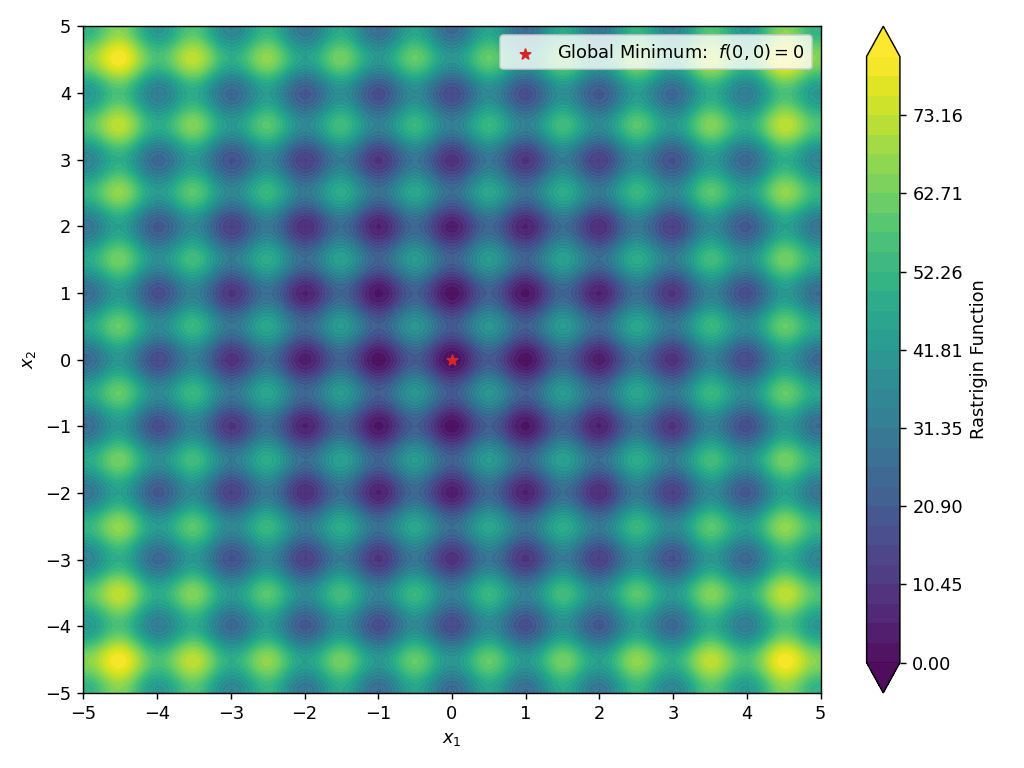
\includegraphics[width=0.5\textwidth]{benchmarks/test_Rastrigin.png}}
	\caption{The Rastrigin function.}
	\label{fig:Rastrigin}
\end{figure}

\begin{figure}[htbp]
	\centerline{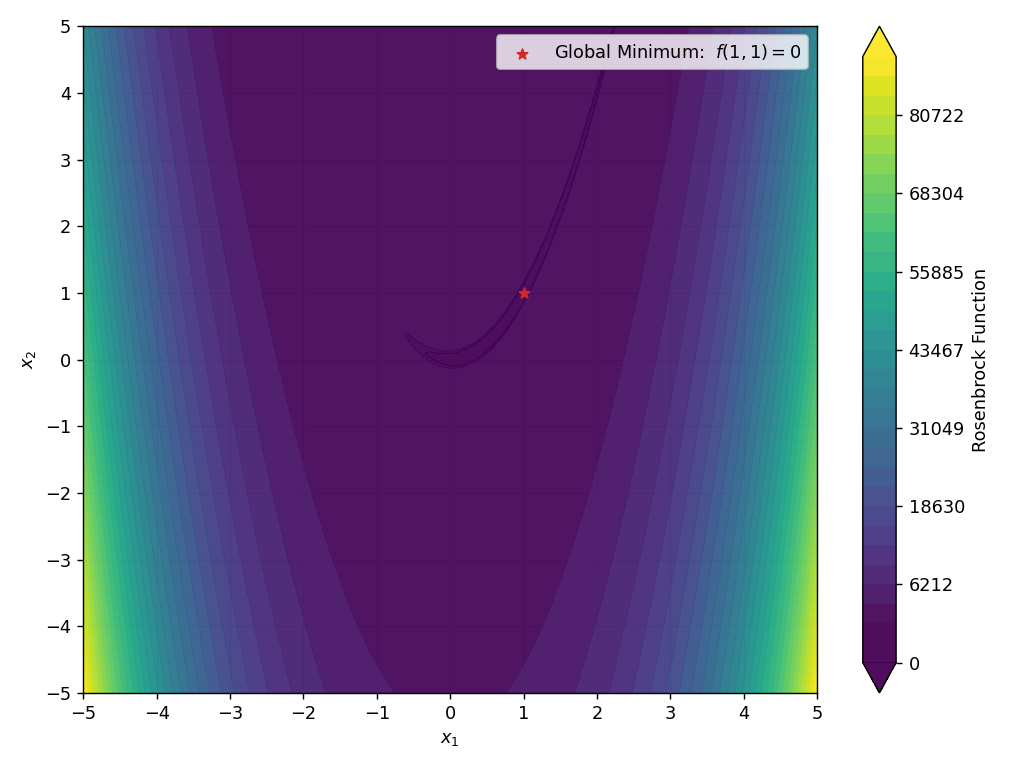
\includegraphics[width=0.5\textwidth]{benchmarks/test_Rosenbrock.png}}
	\caption{The Rosenbrock function.}
	\label{fig:Rosenbrock}
\end{figure}

\begin{figure}[htbp]
	\centerline{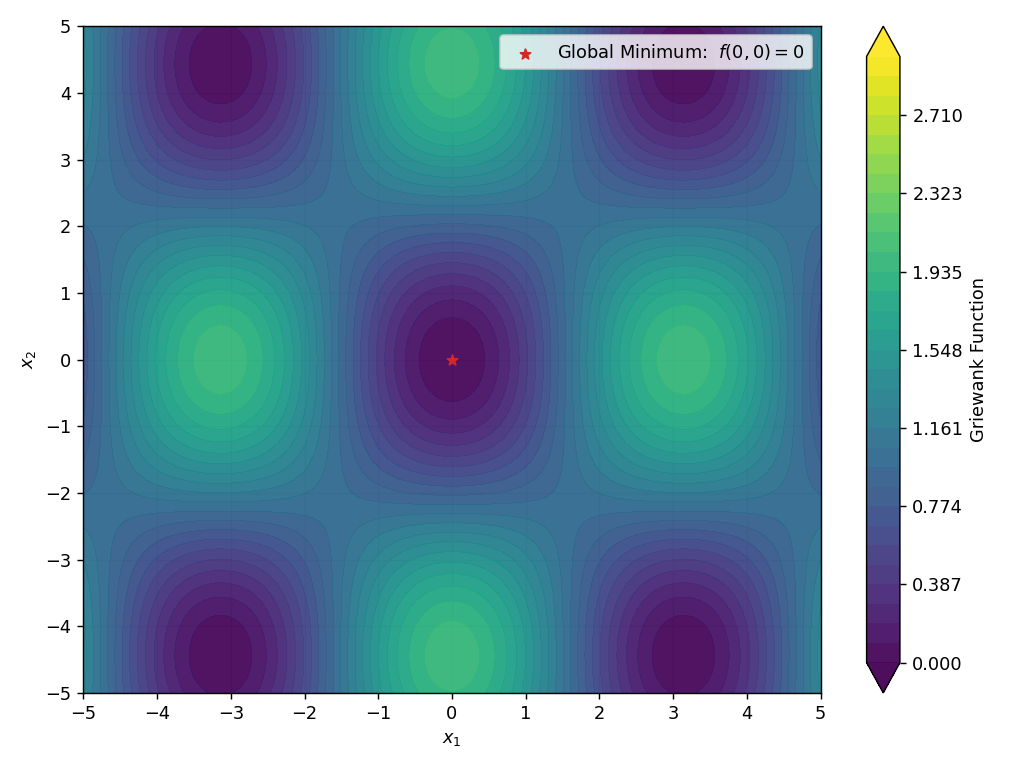
\includegraphics[width=0.5\textwidth]{benchmarks/test_Griewank.png}}
	\caption{The Griewank function.}
	\label{fig:Griewank}
\end{figure}

\begin{figure}[htbp]
	\centerline{\includegraphics[width=0.5\textwidth]{benchmarks/test_Styblinski–Tang.png}}
	\caption{The Styblinski–Tang function.}
	\label{fig:Styblinski–Tang}
\end{figure}

\subsubsection{Surrogate Model}

Given the ubiquity of machine learning surrogate models in the reviewed literature, this work adopts the same approach. In particular, a multilayer perceptron (MLP) with hidden layer architecture

$$ \left(\underbrace{100, 100, \cdots, 100}_{D\;\textrm{times}}\right) $$

\noindent that is, $D$ fully-connected layers of 100 neurons each, is adopted. Model training, validation, and testing are carried out using the functionalities of scikit-learn and PyTorch; for details, refer to the GitHub repo. That said, note that the loss function used in the course of training, validation, and testing is (\ref{eqn:surrogate_error}).

\subsubsection{Monte Carlo}

In order to test (\ref{eqn:efficiency_proposition}) and address question 2, a full factorial Monte Carlo approach is taken. This approach can be summarized in the following pseudocode:

\begin{verbatim}
for benchmark_problem in benchmark_list:
  for sampling_scheme in scheme_list:
    for D in [2, 3, 4, 5, 6]:
      for N in [
      	3D, 4D, 5D, ..., 10D,
      	3^D, 4^D, 5^D, ..., 10^D
      ] up to max of 10^5:
        for trial = 1 ... 50:
          sample objective, get data;
      
          train/test split data;
      
          normalize data;
      
          train surrogate using
            validation/early-stopping;
        
          test surrogate;
        
          compute surrogate efficiency
            using test data;
        
          log results;
\end{verbatim}

\noindent That is, for every combination of benchmark problem, sampling scheme, dimensionality, and number of samples, do 50 Monte Carlo trials of sample (some randomness here), split (some randomness here), train (some randomness here), and test. By way of this approach, a results table with up to $4\times 2\times 5\times 16\times 50 = 32,000$ rows is generated. Note that the ``\texttt{up to max of 10\^{}5}" limit placed on number of samples (for the sake of runtime) is why the results table contains \textit{up to} 32,000 rows; the actual number obtained will be less than this.

\section{Results}

[...]

\section{Discussion}

[...]

\section{Conclusion}

[...]

\section{Future Work}

[...]


%%%% ==== REFERENCES ================================================================ %%%%

\bibliography{/home/primed-anthony/MECH_PhD/tex/refs/refs.bib}{}
\bibliographystyle{IEEEtran}

\end{document}


%%%% ==== TEMPLATES ================================================================= %%%%

\begin{table}[htbp]
	\caption{Table Type Styles}
	\begin{center}
	\begin{tabular}{|c|c|c|c|}
		\hline
		\textbf{Table}&\multicolumn{3}{|c|}{\textbf{Table Column Head}} \\
		\cline{2-4} 
		\textbf{Head} & \textbf{\textit{Table column subhead}}& \textbf{\textit{Subhead}}& 		\textbf{\textit{Subhead}} \\
		\hline
		copy& More table copy$^{\mathrm{a}}$& &  \\
		\hline
		\multicolumn{4}{l}{$^{\mathrm{a}}$Sample of a Table footnote.}
	\end{tabular}
	\label{tab1}
	\end{center}
\end{table}

\begin{figure}[htbp]
	\centerline{
\includegraphics{fig1.png}}
	\caption{Example of a figure caption.}
	\label{fig}
\end{figure}
